\documentclass{standalone}
\usepackage{tikz}
\usepackage{ctex,siunitx}
\setCJKmainfont{Noto Serif CJK SC}
\usepackage{tkz-euclide}
\usepackage{amsmath}
\usetikzlibrary{patterns, calc}
\usetikzlibrary {decorations.pathmorphing, decorations.pathreplacing, decorations.shapes,}
\newcommand\hand[2][0]{
    \begin{scope}[#2,rotate=#1]
    \fill[pink!10!orange!10,draw=black,very thin]
    ( 0.381,-0.532)..controls( 0.381,-0.532)and( 0.453,-0.637)..
    ( 0.528,-0.619)..controls( 0.569,-0.608)and( 0.617,-0.592)..
    ( 0.656,-0.559)..controls( 0.656,-0.559)and( 1.052,-0.743)..
    ( 1.265,-0.543)..controls( 1.265,-0.543)and( 1.394,-0.497)..
    ( 1.530,-0.522)..controls( 1.666,-0.548)and( 1.615, 0.055)..
    ( 1.615, 0.055)..controls( 1.615, 0.055)and( 1.419, 0.062)..
    ( 1.341, 0.100)..controls( 1.264, 0.138)and( 1.192, 0.195)..
    ( 1.000, 0.235)..controls( 0.809, 0.275)and( 0.544, 0.376)..
    ( 0.413, 0.370)..controls( 0.332, 0.366)and(-0.105, 0.228)..
    (-0.166, 0.109)..controls(-0.185, 0.072)and(-0.211,-0.006)..
    (-0.220,-0.076)..controls(-0.220,-0.076)and(-0.256,-0.256)..
    (-0.097,-0.285)..controls(-0.052,-0.297)and(-0.029,-0.260)..
    (-0.019,-0.245)..controls(-0.008,-0.229)and( 0.017,-0.315)..
    ( 0.040,-0.343)..controls( 0.063,-0.371)and( 0.097,-0.440)..
    ( 0.177,-0.440)..controls( 0.191,-0.441)and( 0.207,-0.442)..
    ( 0.223,-0.441)..controls( 0.223,-0.441)and( 0.282,-0.549)..
    ( 0.360,-0.536)..controls( 0.366,-0.535)and( 0.373,-0.534)..cycle;
  \draw[very thin]
  ( 0.752, 0.050)..controls( 0.752, 0.050)and( 0.479, 0.051)..
( 0.359, 0.091)..controls( 0.261, 0.123)and( 0.193, 0.129)..
( 0.071, 0.115)..controls(-0.052, 0.101)and(-0.178, 0.138)..
(-0.141,-0.040)..controls(-0.113,-0.173)and( 0.258,-0.180)..
( 0.337,-0.164)..controls( 0.366,-0.157)and( 0.510,-0.263)..( 0.640,-0.218)
(-0.016,-0.235)..controls( 0.002,-0.204)and( 0.011,-0.164)..( 0.007,-0.146)
(0.223,-0.441)..controls(0.312,-0.438)and(0.422,-0.404)..
(0.468,-0.291)..controls(0.476,-0.269)and(0.360,-0.166)..
(0.240,-0.242)..controls(0.226,-0.233)and(0.205,-0.224)..(0.219,-0.183)
(0.381,-0.532)..controls(0.473,-0.506)and(0.676,-0.401)..
(0.615,-0.331)..controls(0.586,-0.298)and(0.537,-0.260)..(0.472,-0.280)
(0.398,-0.262)..controls(0.420,-0.271)and(0.441,-0.285)..
(0.438,-0.301)..controls(0.435,-0.316)and(0.364,-0.387)..
(0.342,-0.382)..controls(0.344,-0.383)and(0.295,-0.348)..
(0.319,-0.309)..controls(0.343,-0.270)and(0.377,-0.252)..(0.398,-0.262)
(0.566,-0.236)..controls(0.566,-0.236)and(0.675,-0.413)..(1.099,-0.380)
(0.625, 0.066)..controls(0.625, 0.066)and(0.702, 0.114)..(0.801, 0.100)
(0.481, 0.073)..controls(0.481, 0.073)and(0.486, 0.167)..(0.509, 0.222)
(0.353, 0.096)..controls(0.353, 0.096)and(0.332, 0.155)..(0.338, 0.182)
(0.234,-0.017)..controls(0.234,-0.017)and(0.226, 0.063)..(0.233, 0.079)
(0.195,-0.010)..controls(0.195,-0.010)and(0.184, 0.064)..(0.196, 0.091)
(-0.130,-0.034)..controls(-0.130,-0.034)and( 0.023,-0.059)..
( 0.038,-0.028)..controls( 0.053, 0.003)and( 0.077, 0.079)..( 0.039, 0.109)
(0.228,-0.244)..controls(0.228,-0.244)and(0.166,-0.289)..(0.155,-0.319)
(0.318,-0.422)..controls(0.318,-0.422)and(0.266,-0.402)..(0.272,-0.370)
(0.492,-0.481)..controls(0.492,-0.481)and(0.459,-0.463)..(0.451,-0.445)
(0.541,-0.446)..controls(0.541,-0.446)and(0.489,-0.426)..
(0.508,-0.391)..controls(0.526,-0.356)and(0.565,-0.321)..(0.593,-0.328)
(0.656,-0.559)..controls(0.688,-0.532)and(0.715,-0.493)..
(0.728,-0.438)..controls(0.731,-0.403)and(0.666,-0.363)..(0.630,-0.386)
(0.687,-0.517)..controls(0.687,-0.517)and(0.613,-0.515)..
(0.631,-0.476)..controls(0.649,-0.438)and(0.666,-0.395)..(0.703,-0.399)
(0.636,-0.566)..controls(0.636,-0.566)and(0.602,-0.557)..(0.587,-0.522)
(1.329,-0.381)..controls(1.329,-0.381)and(1.481,-0.291)..(1.489,-0.356);
  \end{scope}
}
\begin{document}
\small
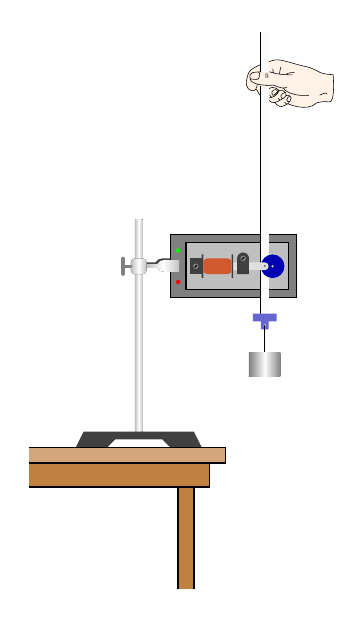
\begin{tikzpicture}[>=stealth,scale=1.0]
  \hand{xshift=-1mm,scale=0.6}
  \fill[darkgray](-1.1,-2.3)--(-1.3,-2.3)arc(90:150:0.1)--(-1.5,-2.35)--(-1.5,-2.4)--(-1.1,-2.4);
  \draw[fill=gray](0.4,-2.8)rectangle(-1.2,-2.0);
  \draw[fill=lightgray](0.3,-2.7)rectangle(-1.0,-2.1);
  \draw[double=black!2,line width=0.1mm,double distance=1mm](0,0.07)--++(0,0.5)(0,-0.11)--(0,-3);
  \fill[blue!70!black](0.1,-2.4)circle(0.15);
  \fill[ball color=white](0.1,-2.4)circle(0.5pt);
  \fill[lightgray!50](-0.5,-2.45)--(0,-2.45)arc(-90:90:0.05)--(-0.5,-2.35);
  \fill[ball color=gray](0,-2.4)circle(0.3pt);
  \fill[darkgray](-0.35,-2.5)--(-0.2,-2.5)--(-0.2,-2.3)arc(0:180:0.075)--cycle;
  \fill[gray](-0.275,-2.3)circle(1pt);
  \draw[line cap =round]([shift=(-135:0.5pt)]-0.275,-2.3)--++(45:1pt);
  \fill[darkgray](-0.4,-2.55)rectangle(-0.42,-2.25)(-0.78,-2.55)rectangle(-0.8,-2.25);
  \fill[red!30!brown,rounded corners=0.5mm](-0.78,-2.5)rectangle(-0.42,-2.3);
  \fill[darkgray](-0.95,-2.5)rectangle(-0.8,-2.3);
  \fill[red](-1.1,-2.6)circle(0.8pt);
  \fill[green](-1.1,-2.2)circle(0.8pt);
  \fill[gray](-0.875,-2.4)circle(1pt);
  \draw[line cap =round]([shift=(-135:0.5pt)]-0.875,-2.4)--++(45:1pt);
  \fill[blue!70!black!60,even odd rule](0,-3)--++(-0.15,0)--++(0,-0.1)--++(0.1,0)--++(0,-0.1)--++(0.1,0)--++(0,0.1)--++(0.1,0)--++(0,0.1)--cycle(0,-3.15)circle(0.5pt);
  \draw(0,-3.15)--(0,-3.5);
  \fill[left color=gray,right color=gray,middle color=white](-0.2,-3.5)rectangle(0.2,-3.8);
  \fill[left color=lightgray,right color=lightgray,middle color=white](-1.08,-2.32)--(-1.28,-2.32)arc(90:150:0.1)--(-1.5,-2.37)--(-1.5,-2.42)--(-1.367,-2.42)arc(210:270:0.1)--(-1.08,-2.47);
  \fill[left color=lightgray,right color=lightgray,middle color=white](-1.65,-1.8)rectangle(-1.55,-4.5);
  \fill[left color=lightgray,right color=lightgray,middle color=white,rounded corners=0.5mm](-1.5,-2.3)rectangle(-1.7,-2.5);
  \draw[very thick,gray,line cap=round](-1.7,-2.4)--++(-0.1,0)(-1.8,-2.5)--++(0,0.2);
  % \fill[darkgray](-0.8,-4.5)rectangle(-2.4,-4.7);
  \fill[darkgray](-0.9,-4.5)--(-0.8,-4.7)--(-1.2,-4.7)--(-1.3,-4.6)--(-1.9,-4.6)--(-2,-4.7)--(-2.4,-4.7)--(-2.3,-4.5)--cycle;
  \draw [semithick,fill=brown!70](-3,-4.7)--(-0.5,-4.7)--(-0.5,-4.9)--(-3,-4.9);
  \draw [semithick,fill=brown](-3,-4.9)--(-0.7,-4.9)--(-0.7,-5.2)--(-3,-5.2);
  \draw [semithick,fill=brown](-1.1,-6.5)--(-1.1,-5.2)--(-0.9,-5.2)--(-0.9,-6.5);
\end{tikzpicture}
\end{document}